\section{Transactions}

\begin{definition}
    A \emph{transaction} is an elementary, atomic unit of work performed by an application. 
    Each transaction is conceptually encapsulated within two commands:
    \begin{itemize}
        \item Begin transaction.
        \item End transaction.
    \end{itemize}
\end{definition}
In the context of a transaction, the conclusion of the process is indicated by executing one of the following commands: either commit or rollback.
\begin{definition}
    The \emph{On-Line Transaction Processing} (OLTP) is a system that supports the execution of transactions on behalf of concurrent applications. 
\end{definition}
The application has the capability to execute multiple transactions, with transactions being an integral part of the application rather than the other way around. 
These transactions adhere to the ACID properties:
\begin{enumerate}
    \item Atomicity: a transaction represents an indivisible unit of execution, ensuring that either all operations within the transaction are executed or none at all.
        The commitment of the transaction, marked by the execution of the commit command, signifies the successful conclusion. 
        Any error occurring before the commit should trigger a rollback, and errors occurring afterward should not impact the transaction.        
        The rollback can be initiated by either a rollback statement or the Database Management System (DBMS).
        In the event of a rollback, the executed work must be undone, restoring the database to its state before the transaction's initiation.
        It becomes the responsibility of the application to determine whether an aborted transaction needs to be redone.
    \item Consistency: transactions must adhere to the integrity constraints of the database.
        If the initial state $S_0$ is consistent, the final state $S_f$ must also be consistent. 
        This consistency requirement, however, does not necessarily extend to intermediate states $S_i$.
    \item Isolation: the execution of a transaction must remain independent of concurrently executing transactions. 
        This ensures that the outcome of one transaction does not affect the execution of others.
    \item Durability: the effects of a successfully committed transaction are permanent, enduring indefinitely and remaining unaffected by any system faults.
\end{enumerate}
\begin{table}[H]
    \centering
    \begin{tabular}{c|c|c}
    \textbf{Property} & \textbf{Actions}       & \textbf{Architectural element} \\ \hline
    Atomicity         & Abort-rollback-restart & Query Manager                  \\
    Consistency       & Integrity checking     & Integrity Control System       \\
    Isolation         & Concurrency control    & Concurrency Control System     \\
    Durability        & Recovery management    & Reliability Manager           
    \end{tabular}
\end{table}
\begin{figure}[H]
    \centering
    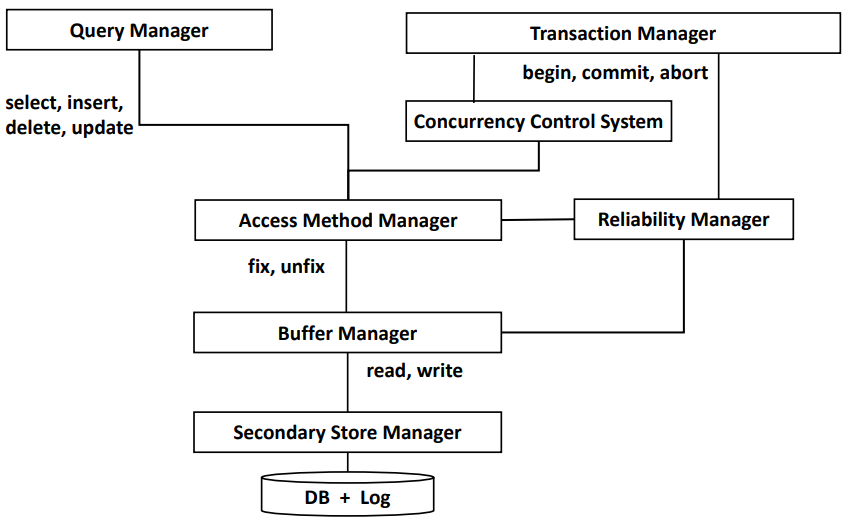
\includegraphics[width=0.75\linewidth]{images/architecture.png}
    \caption{Architecture of a Data Base Management System}
\end{figure}